\documentclass{standalone}
\usepackage{tikz}
\usepackage{textcomp}

\begin{document}

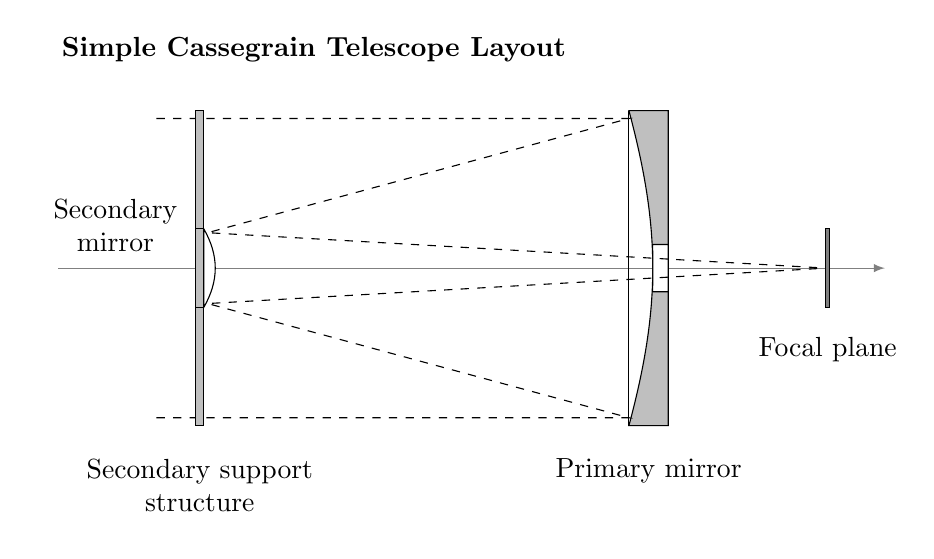
\begin{tikzpicture}

    \draw[gray, -latex] (-1.25,0) -- (9.25,0);

    \node[above] at (2,2.5) {\textbf{Simple Cassegrain Telescope Layout}};
    % secondary
    \draw[fill=white] (0.6,0.5) to[bend left] (0.6,-0.5) -- cycle;
    \draw[fill=lightgray] (0.6,0.5) -- (0.6,-0.5) -- (0.5,-0.5) -- (0.5,0.5) -- cycle;
    \node [left] at (0.6,0.5) {\begin{tabular}{c}Secondary\\mirror\end{tabular}};

    % primary
    \draw[fill=lightgray] (6,2) to[out=-75,in=75] (6,-2) -- (6.5,-2) -- (6.5,2) -- cycle;
    \draw (6,2) -- (6,-2);
    \node [below] at (6.25,-2.3) {Primary mirror};

    % primary hole
    \draw[fill=white] (6.3,0.3) to[out=-88.5,in=88.5] (6.3,-0.3) -- (6.5,-0.3) -- (6.5,0.3) -- cycle;

    \draw[dashed] (0,1.9) -- (6,1.9) -- (0.65,0.45) -- (8.5,0);
    \draw[dashed] (0,-1.9) -- (6,-1.9) -- (0.65,-0.45) -- (8.5,0);

    % spiders
    \draw[fill=lightgray] (0.5,0.5) -- (0.5,2) -- (0.6,2) -- (0.6,0.5) -- cycle;
    \draw[fill=lightgray] (0.5,-0.5) -- (0.5,-2) -- (0.6,-2) -- (0.6,-0.5) -- cycle;
    \node [below] at (0.55, -2.25) {\begin{tabular}{c}Secondary support \\ structure\end{tabular}};

    % focal plane
    \draw[fill=gray] (8.5,0.5) -- (8.55,0.5) -- (8.55,-0.5) -- (8.5,-0.5) -- cycle;
    \node [below] at (8.525,-0.75) {Focal plane};



\end{tikzpicture}
\end{document}
